\chapter{Camps magnètics d'espires i bobines}
\begin{resum}
Aquesta pràctica té com a objectiu principal l'estudi dels camps magnètics creats per diferents configuracions d'espires i bobines. Mitjançant una sonda Hall s'han mesurat els camps creats, al seu centre, per espires de radis diferents, així com per conjunts d'una, dues i tres espires. De la mateixa manera s'han realitzat mesures del camp magnètic al llarg de l'eix de bobinas de diversos radis.

Amb les dades experimentals s'ha posat a prova la dependència del camp magnètic d'una espira del seu radi i també del nombre d'espires, tal i com prediu la llei de Biot-Savart. També s'ha pogut trobar un valor per a la permeabilitat magnètica del buit, \( \mu_0 \) amb un error relatiu del $12\%$.
\end{resum}


\section{Introducció}
En la primera part de la pràctica s'estudiarà el camp magnètic degut a conjunts d'espires. Si considerem un conjunt de \( N \) espires de radi \( R \) per les que hi circula un corrent constant \( I \), un càlcul elemental amb la llei de Biot-Savart ens dóna que el camp magnètic \( \vec{B} \) al seu centre és
\begin{equation}\label{eq:camp espira}
  \vec{B}=\frac{\mu_0 I N}{2 R}\vec{e}_z,
\end{equation}
on \( \vec{e}_z \) és el vector unitari perpendicular al pla de les espires. Així doncs esperem poder observar les relacions \( B \propto R^{-1} \) i \( B \propto N \). 

Pel que fa al camp magnètic d'una bobina, sabem que en el cas d'una bobina infinita el camp en el seu interior és constant i nul a l'exterior. En el cas d'una bobina finita de longitud \( L \), radi \( R \), \( N \) voltes i per la qual hi passa una intensitat constant \( I \), el camp a punts del seu eix es pot trobar de manera exacta mitjançant la llei de Biot-Savart i resulta
\begin{equation}\label{eq:camp bobina}
  \vec{B}=\frac{\mu_0 I N}{2 L}\left(\frac{z + L/2}{\sqrt{R^2+(z+L/2)^2}} - \frac{z - L/2}{\sqrt{R^2 + (z - L/2)^2}}\right) \vec{e}_z,
\end{equation}
on \( z \) és la posició de la sonda al llarg de l'eix de la bobina ---fixant \( z = 0 \) al seu centre--- i \( \vec{e}_z \) és el vector unitari para\l.lel a l'eix. Quan \( L \gg R \) aleshores l'\cref{eq:camp bobina} dóna lloc a un camp que és gairebé constant per \( \abs{z} < L/2 \) i que decau molt depressa cap a 0 quan \( \abs{z} > L/2 \). 

\section{Mètode experimental}
\subsection{Espires}
Per a realitzar les mesures s'ha fet servir la disposició que es mostra a la \cref{fig:circuit teslametre}. Les espires i la sonda estaven cada una sobre un suport de manera que la sonda estigués a la mateixa alçada que el centre de l'espira. La sonda també estava muntada sobre una rail de manera que es mantingués sempre sobre l'eix perpendicular de les espires.

\begin{figure}[htb]
  \centering \small \sffamily
  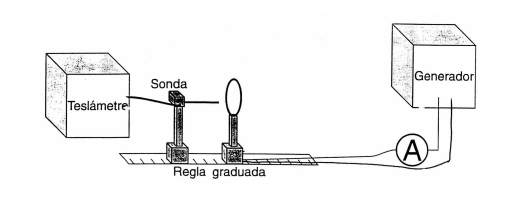
\includegraphics{circuit-teslametre.png}
  \caption{Esquema del circuit emprat per a mesurar el camp magnètic}
  \label{fig:circuit teslametre}
\end{figure}

El corrent subministrat per la font es va fixar a \SI{4.00}{A} i tot seguit la sonda es va desplaçar fins al centre de l'espira ---de la qual ja s'havia mesurat el radi---. Cal mencionar que el sensor de camp magnètic no es troba exactament a la punta de la sonda, de manera que és complicat determinar exactament quan és que efectivament s'estava mesurant el camp al centre. Com que, d'acord amb el resultat teòric, el camp magnètic s'una espira és màxim al seu centre, es va considerar el màxim valor registrat pel teslàmetre. Degut a la seva alta sensibilitat, el teslàmetre trigava un temps considerable a estabilitzar la seva lectura després de canvis bruscos en el camp magnètic. 

S'han pres sis mesures del camp per a cada espira---tres en total, cada una amb un radi diferent. Tres amb un sentit del corrent i tres amb el corrent en sentit oposat. Aleshores s'ha fet el promig de les sis lectures per a minimitzar errors aleatoris deguts a fluctuacions en la mesura del teslàmetre.   

Posteriorment s'ha mesurat el camp al centre del conjunt de 1, 2 i 3 espires seguint el mateix procediment.

\subsection{Bobines}
Per la mesura del camp a l'interior de les bobines s'ha fet servir el mateix circuit que es mostra a la \cref{fig:circuit teslametre}.

Ajustant la intensitat a \data{1.00}{0.01}{A} a l'amperímetre, s'ha mesurat el camp a diversos punts a l'interior de la bobina. Per fer-ho s'ha ajustat l'alçada de la sonda de manera que aquesta quedi sobre l'eix de la bobina. Començant pel punt immediatament a l'exterior de la bobina s'ha fet avançar la sonda sobre el regle mesurant el camp cada \SI{3}{cm} de manera que n'han resultat 8 mesures a diferents punts de l'eix.

Aquest mateix procediment s'ha repetit per cada una de les bobines diferents.  

\section{Resultats}
\subsection{Espires}\label{sec:espires}
Com s'ha mencionat anteriorment, en aquesta secció es presenten els resultats relatius a la part de la pràctica referent a les espires. A la \cref{tab:camp espires en funcio de r} es presenten les mesures del camp magnètic al centre d'una espira en funció del seu radi. 

\begin{table}[htb]
  \centering \small \sffamily
  \caption{Taula de valors teòrics i experimentals}
  \label{tab:camp espires en funcio de r}
	\begin{tabular}{SSS}
		\toprule
		{Radi (\data{}{0.2}{cm})} & { \( B_{\textsf{exp}}\ (\SI{d-5}{T}) \) } & { \( B_{\textsf{teò}}\ (\SI{d-5}{T}) \) } \\
		\midrule
		3.0 & 7.3\pm1.4 & 8.4\pm0.4 \\
		4.3 & 6.0\pm1.6 & 5.9\pm0.2 \\
		6.0 & 5.0\pm1.6 & 4.2\pm0.1 \\
		\bottomrule
	\end{tabular}
\end{table}

Les incerteses dels camps experimentals de la \cref{tab:camp espires en funcio de r} han estat calculades segons la desviació estàndard de les diferents mesures realitzades. Pel que fa a les incerteses teòriques, aquestes han estat calculades per propagació d'incerteses de la fórmula \cref{eq:camp espira}. Com podem veure en els tres casos, els valors experimentals amb els seus respectius intervals d'incertesa coincideixen en alguns punts amb els valors teòrics i els seus intervals, per tant els resultats són compatibles. Es pot observar que l'incertesa dels resultats experimentals és considerablement major. Això és degut a les imprecisions dels aparells emprats per a la mesura dels camps, especialment a les contínues fluctuacions del teslàmetre. 

Tanmateix, el fet més rellevant que podem observar és la disminució del camp a l'interior de l'espira a mesura que augmenta el seu radi. Aquest resultat ja era el que esperavem teòricament. Per fer més èmfasi en aquest fet es presenta la gràfica de la figura cref{fig:camp espira}, on es representa el camp magnètic al centre en funció del radi de l'espira.
\begin{figure}[htb]
  \centering
	% GNUPLOT: LaTeX picture with Postscript
\begingroup
\sffamily \small
  \makeatletter
  \providecommand\color[2][]{%
    \GenericError{(gnuplot) \space\space\space\@spaces}{%
      Package color not loaded in conjunction with
      terminal option `colourtext'%
    }{See the gnuplot documentation for explanation.%
    }{Either use 'blacktext' in gnuplot or load the package
      color.sty in LaTeX.}%
    \renewcommand\color[2][]{}%
  }%
  \providecommand\includegraphics[2][]{%
    \GenericError{(gnuplot) \space\space\space\@spaces}{%
      Package graphicx or graphics not loaded%
    }{See the gnuplot documentation for explanation.%
    }{The gnuplot epslatex terminal needs graphicx.sty or graphics.sty.}%
    \renewcommand\includegraphics[2][]{}%
  }%
  \providecommand\rotatebox[2]{#2}%
  \@ifundefined{ifGPcolor}{%
    \newif\ifGPcolor
    \GPcolortrue
  }{}%
  \@ifundefined{ifGPblacktext}{%
    \newif\ifGPblacktext
    \GPblacktextfalse
  }{}%
  % define a \g@addto@macro without @ in the name:
  \let\gplgaddtomacro\g@addto@macro
  % define empty templates for all commands taking text:
  \gdef\gplbacktext{}%
  \gdef\gplfronttext{}%
  \makeatother
  \ifGPblacktext
    % no textcolor at all
    \def\colorrgb#1{}%
    \def\colorgray#1{}%
  \else
    % gray or color?
    \ifGPcolor
      \def\colorrgb#1{\color[rgb]{#1}}%
      \def\colorgray#1{\color[gray]{#1}}%
      \expandafter\def\csname LTw\endcsname{\color{white}}%
      \expandafter\def\csname LTb\endcsname{\color{black}}%
      \expandafter\def\csname LTa\endcsname{\color{black}}%
      \expandafter\def\csname LT0\endcsname{\color[rgb]{1,0,0}}%
      \expandafter\def\csname LT1\endcsname{\color[rgb]{0,1,0}}%
      \expandafter\def\csname LT2\endcsname{\color[rgb]{0,0,1}}%
      \expandafter\def\csname LT3\endcsname{\color[rgb]{1,0,1}}%
      \expandafter\def\csname LT4\endcsname{\color[rgb]{0,1,1}}%
      \expandafter\def\csname LT5\endcsname{\color[rgb]{1,1,0}}%
      \expandafter\def\csname LT6\endcsname{\color[rgb]{0,0,0}}%
      \expandafter\def\csname LT7\endcsname{\color[rgb]{1,0.3,0}}%
      \expandafter\def\csname LT8\endcsname{\color[rgb]{0.5,0.5,0.5}}%
    \else
      % gray
      \def\colorrgb#1{\color{black}}%
      \def\colorgray#1{\color[gray]{#1}}%
      \expandafter\def\csname LTw\endcsname{\color{white}}%
      \expandafter\def\csname LTb\endcsname{\color{black}}%
      \expandafter\def\csname LTa\endcsname{\color{black}}%
      \expandafter\def\csname LT0\endcsname{\color{black}}%
      \expandafter\def\csname LT1\endcsname{\color{black}}%
      \expandafter\def\csname LT2\endcsname{\color{black}}%
      \expandafter\def\csname LT3\endcsname{\color{black}}%
      \expandafter\def\csname LT4\endcsname{\color{black}}%
      \expandafter\def\csname LT5\endcsname{\color{black}}%
      \expandafter\def\csname LT6\endcsname{\color{black}}%
      \expandafter\def\csname LT7\endcsname{\color{black}}%
      \expandafter\def\csname LT8\endcsname{\color{black}}%
    \fi
  \fi
    \setlength{\unitlength}{0.0500bp}%
    \ifx\gptboxheight\undefined%
      \newlength{\gptboxheight}%
      \newlength{\gptboxwidth}%
      \newsavebox{\gptboxtext}%
    \fi%
    \setlength{\fboxrule}{0.5pt}%
    \setlength{\fboxsep}{1pt}%
\begin{picture}(5668.00,3400.00)%
    \gplgaddtomacro\gplbacktext{%
      \csname LTb\endcsname%%
      \put(814,704){\makebox(0,0)[r]{\strut{}\num{30}}}%
      \put(814,1117){\makebox(0,0)[r]{\strut{}\num{40}}}%
      \put(814,1529){\makebox(0,0)[r]{\strut{}\num{50}}}%
      \put(814,1942){\makebox(0,0)[r]{\strut{}\num{60}}}%
      \put(814,2354){\makebox(0,0)[r]{\strut{}\num{70}}}%
      \put(814,2767){\makebox(0,0)[r]{\strut{}\num{80}}}%
      \put(814,3179){\makebox(0,0)[r]{\strut{}\num{90}}}%
      \put(946,484){\makebox(0,0){\strut{}\num{16}}}%
      \put(1379,484){\makebox(0,0){\strut{}\num{18}}}%
      \put(1811,484){\makebox(0,0){\strut{}\num{20}}}%
      \put(2244,484){\makebox(0,0){\strut{}\num{22}}}%
      \put(2676,484){\makebox(0,0){\strut{}\num{24}}}%
      \put(3109,484){\makebox(0,0){\strut{}\num{26}}}%
      \put(3541,484){\makebox(0,0){\strut{}\num{28}}}%
      \put(3974,484){\makebox(0,0){\strut{}\num{30}}}%
      \put(4406,484){\makebox(0,0){\strut{}\num{32}}}%
      \put(4839,484){\makebox(0,0){\strut{}\num{34}}}%
      \put(5271,484){\makebox(0,0){\strut{}\num{36}}}%
      \put(3974,1117){\makebox(0,0){\strut{}$r^2 =$ \num{0.999}}}%
    }%
    \gplgaddtomacro\gplfronttext{%
      \csname LTb\endcsname%%
      \put(198,1941){\rotatebox{-270}{\makebox(0,0){\strut{}$\mathsf{B \ (\si{\micro T})}$}}}%
      \put(3108,154){\makebox(0,0){\strut{}$\mathsf{1/r \ (\si{m^{-1}})}$}}%
    }%
    \gplbacktext
    \put(0,0){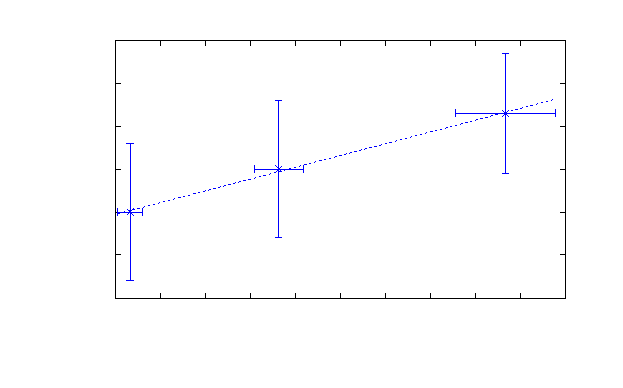
\includegraphics{camp-radi}}%
    \gplfronttext
  \end{picture}%
\endgroup

  \caption{Camp magnètic al centre en funció del radi de l'espira}
  \label{fig:camp espira}
\end{figure}

Com es pot observar a la regressió de la figura \cref{fig:camp espira}, la dependència del camp magnètic amb l'invers del radi és lineal amb $r^2=0.999$. És a dir el camp magnètic decau com \( \frac{1}{R} \). Tot i així el fet que només s'hagi mesurat el camp per a tres radis diferents, fa que no es pugui afirmar amb rotunditat que aquest és sempre el comportament del camp magnètic. Tanmateix, això és el que semblen indicar les dades experimentals.

La taula \cref{tab:camp espires en funcio de n} presenta els camp magnètics teòrics i experimentals al centre dels conjunts de 1, 2 i 3 espires. 

\begin{table}[htb]
	\centering \small \sffamily
	\caption{Valors teòrics i experimentals del camp magnètic al centre d'un conjunt de \( N \) espires}
	\label{tab:camp espires en funcio de n}
	\begin{tabular}{SSS}
		\toprule
		{Nombre d'espires \( N \)} & { \( B_{\textsf{exp}}\ (\SI{d-5}{T}) \) } & { \( B_{\textsf{teò}}\ (\SI{d-5}{T}) \) } \\
		\midrule
		1 & 5.0\pm1.6 & 4.2\pm0.1 \\
		2 & 8.8\pm1.5 & 8.4\pm0.2 \\
		3 & 12.3\pm1.5 & 12.6\pm0.3 \\
		\bottomrule
	\end{tabular}
\end{table}

Podem observar que en aquest cas els intervals dels camps teòrics i experimentals també se solapen i per tant les observacions satisfan l'esperat. Altra vegada tornem a tenir incerteses majors pels valors experimentals pel mateix fet anteriorment mencionat. Els resultats ens permeten observar que com més espires introduïm al conjunt més intens es torna el camp al centre d'aquest. Aquesta dependència es pot observar clarament al gràfic experimental del camp al centre en funció del nombre d'espires que s'exposa a la \cref{fig:camp vs n}.

\begin{figure}[htb]
  \centering
	% GNUPLOT: LaTeX picture with Postscript
\begingroup
\sffamily \small
  \makeatletter
  \providecommand\color[2][]{%
    \GenericError{(gnuplot) \space\space\space\@spaces}{%
      Package color not loaded in conjunction with
      terminal option `colourtext'%
    }{See the gnuplot documentation for explanation.%
    }{Either use 'blacktext' in gnuplot or load the package
      color.sty in LaTeX.}%
    \renewcommand\color[2][]{}%
  }%
  \providecommand\includegraphics[2][]{%
    \GenericError{(gnuplot) \space\space\space\@spaces}{%
      Package graphicx or graphics not loaded%
    }{See the gnuplot documentation for explanation.%
    }{The gnuplot epslatex terminal needs graphicx.sty or graphics.sty.}%
    \renewcommand\includegraphics[2][]{}%
  }%
  \providecommand\rotatebox[2]{#2}%
  \@ifundefined{ifGPcolor}{%
    \newif\ifGPcolor
    \GPcolortrue
  }{}%
  \@ifundefined{ifGPblacktext}{%
    \newif\ifGPblacktext
    \GPblacktextfalse
  }{}%
  % define a \g@addto@macro without @ in the name:
  \let\gplgaddtomacro\g@addto@macro
  % define empty templates for all commands taking text:
  \gdef\gplbacktext{}%
  \gdef\gplfronttext{}%
  \makeatother
  \ifGPblacktext
    % no textcolor at all
    \def\colorrgb#1{}%
    \def\colorgray#1{}%
  \else
    % gray or color?
    \ifGPcolor
      \def\colorrgb#1{\color[rgb]{#1}}%
      \def\colorgray#1{\color[gray]{#1}}%
      \expandafter\def\csname LTw\endcsname{\color{white}}%
      \expandafter\def\csname LTb\endcsname{\color{black}}%
      \expandafter\def\csname LTa\endcsname{\color{black}}%
      \expandafter\def\csname LT0\endcsname{\color[rgb]{1,0,0}}%
      \expandafter\def\csname LT1\endcsname{\color[rgb]{0,1,0}}%
      \expandafter\def\csname LT2\endcsname{\color[rgb]{0,0,1}}%
      \expandafter\def\csname LT3\endcsname{\color[rgb]{1,0,1}}%
      \expandafter\def\csname LT4\endcsname{\color[rgb]{0,1,1}}%
      \expandafter\def\csname LT5\endcsname{\color[rgb]{1,1,0}}%
      \expandafter\def\csname LT6\endcsname{\color[rgb]{0,0,0}}%
      \expandafter\def\csname LT7\endcsname{\color[rgb]{1,0.3,0}}%
      \expandafter\def\csname LT8\endcsname{\color[rgb]{0.5,0.5,0.5}}%
    \else
      % gray
      \def\colorrgb#1{\color{black}}%
      \def\colorgray#1{\color[gray]{#1}}%
      \expandafter\def\csname LTw\endcsname{\color{white}}%
      \expandafter\def\csname LTb\endcsname{\color{black}}%
      \expandafter\def\csname LTa\endcsname{\color{black}}%
      \expandafter\def\csname LT0\endcsname{\color{black}}%
      \expandafter\def\csname LT1\endcsname{\color{black}}%
      \expandafter\def\csname LT2\endcsname{\color{black}}%
      \expandafter\def\csname LT3\endcsname{\color{black}}%
      \expandafter\def\csname LT4\endcsname{\color{black}}%
      \expandafter\def\csname LT5\endcsname{\color{black}}%
      \expandafter\def\csname LT6\endcsname{\color{black}}%
      \expandafter\def\csname LT7\endcsname{\color{black}}%
      \expandafter\def\csname LT8\endcsname{\color{black}}%
    \fi
  \fi
    \setlength{\unitlength}{0.0500bp}%
    \ifx\gptboxheight\undefined%
      \newlength{\gptboxheight}%
      \newlength{\gptboxwidth}%
      \newsavebox{\gptboxtext}%
    \fi%
    \setlength{\fboxrule}{0.5pt}%
    \setlength{\fboxsep}{1pt}%
\begin{picture}(5668.00,3400.00)%
    \gplgaddtomacro\gplbacktext{%
      \csname LTb\endcsname%%
      \put(946,704){\makebox(0,0)[r]{\strut{}\num{20}}}%
      \put(946,1117){\makebox(0,0)[r]{\strut{}\num{40}}}%
      \put(946,1529){\makebox(0,0)[r]{\strut{}\num{60}}}%
      \put(946,1942){\makebox(0,0)[r]{\strut{}\num{80}}}%
      \put(946,2354){\makebox(0,0)[r]{\strut{}\num{100}}}%
      \put(946,2767){\makebox(0,0)[r]{\strut{}\num{120}}}%
      \put(946,3179){\makebox(0,0)[r]{\strut{}\num{140}}}%
      \put(2126,484){\makebox(0,0){\strut{}\num{1}}}%
      \put(3175,484){\makebox(0,0){\strut{}\num{2}}}%
      \put(4223,484){\makebox(0,0){\strut{}\num{3}}}%
      \put(4642,910){\makebox(0,0){\strut{}$r^2 =$ \num{1.000}}}%
    }%
    \gplgaddtomacro\gplfronttext{%
      \csname LTb\endcsname%%
      \put(198,1941){\rotatebox{-270}{\makebox(0,0){\strut{}$\mathsf{B \ (\si{\micro T})}$}}}%
      \put(3174,154){\makebox(0,0){\strut{}$\mathsf{N}$}}%
    }%
    \gplbacktext
    \put(0,0){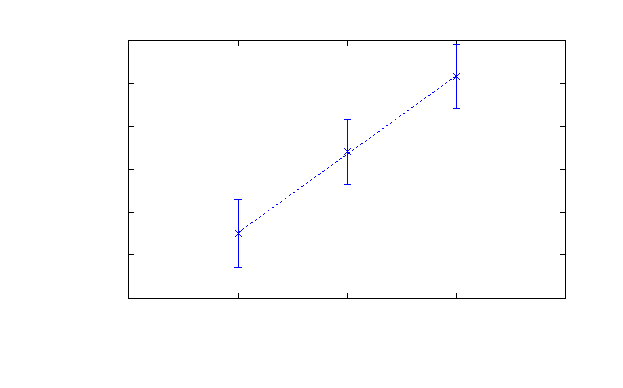
\includegraphics{camp-n}}%
    \gplfronttext
  \end{picture}%
\endgroup

  \caption{Camp al centre en funció del nombre d'espires}
  \label{fig:camp vs n}
\end{figure}

Podem veure a la regressió de la \cref{fig:camp vs n} que aquesta dependència és lineal, amb $r^2=1.000$, com s'esperava dels valors teòrics obtinguts a partir de la \cref{eq:camp espira}. El valor de $\mu_{0}$ obtingut a partir de la regressió tenint en compte que el pendent segons \cref{eq:camp espira} és $\frac{\mu_{0}I}{2R}$  s'obté un valor de $\mu_{0} = \data{1.10}{0.37d-6}{N.A^{-2}} $ que és compatible amb el valor teòric de $\mu_{0}\approx \SI{1.26d-6}{N.A^{-2}} $. Així doncs, vist que el camp augmenta de manera directament proporcional al nombre d'espires, els resultats d'aquest apartat queden interpretats.

\subsection{Bobines}\label{sec:bobines}
\begin{figure}[tp]
	\sffamily \small
	\centering
	% GNUPLOT: LaTeX picture with Postscript
\begingroup
\sffamily \small
  \makeatletter
  \providecommand\color[2][]{%
    \GenericError{(gnuplot) \space\space\space\@spaces}{%
      Package color not loaded in conjunction with
      terminal option `colourtext'%
    }{See the gnuplot documentation for explanation.%
    }{Either use 'blacktext' in gnuplot or load the package
      color.sty in LaTeX.}%
    \renewcommand\color[2][]{}%
  }%
  \providecommand\includegraphics[2][]{%
    \GenericError{(gnuplot) \space\space\space\@spaces}{%
      Package graphicx or graphics not loaded%
    }{See the gnuplot documentation for explanation.%
    }{The gnuplot epslatex terminal needs graphicx.sty or graphics.sty.}%
    \renewcommand\includegraphics[2][]{}%
  }%
  \providecommand\rotatebox[2]{#2}%
  \@ifundefined{ifGPcolor}{%
    \newif\ifGPcolor
    \GPcolortrue
  }{}%
  \@ifundefined{ifGPblacktext}{%
    \newif\ifGPblacktext
    \GPblacktextfalse
  }{}%
  % define a \g@addto@macro without @ in the name:
  \let\gplgaddtomacro\g@addto@macro
  % define empty templates for all commands taking text:
  \gdef\gplbacktext{}%
  \gdef\gplfronttext{}%
  \makeatother
  \ifGPblacktext
    % no textcolor at all
    \def\colorrgb#1{}%
    \def\colorgray#1{}%
  \else
    % gray or color?
    \ifGPcolor
      \def\colorrgb#1{\color[rgb]{#1}}%
      \def\colorgray#1{\color[gray]{#1}}%
      \expandafter\def\csname LTw\endcsname{\color{white}}%
      \expandafter\def\csname LTb\endcsname{\color{black}}%
      \expandafter\def\csname LTa\endcsname{\color{black}}%
      \expandafter\def\csname LT0\endcsname{\color[rgb]{1,0,0}}%
      \expandafter\def\csname LT1\endcsname{\color[rgb]{0,1,0}}%
      \expandafter\def\csname LT2\endcsname{\color[rgb]{0,0,1}}%
      \expandafter\def\csname LT3\endcsname{\color[rgb]{1,0,1}}%
      \expandafter\def\csname LT4\endcsname{\color[rgb]{0,1,1}}%
      \expandafter\def\csname LT5\endcsname{\color[rgb]{1,1,0}}%
      \expandafter\def\csname LT6\endcsname{\color[rgb]{0,0,0}}%
      \expandafter\def\csname LT7\endcsname{\color[rgb]{1,0.3,0}}%
      \expandafter\def\csname LT8\endcsname{\color[rgb]{0.5,0.5,0.5}}%
    \else
      % gray
      \def\colorrgb#1{\color{black}}%
      \def\colorgray#1{\color[gray]{#1}}%
      \expandafter\def\csname LTw\endcsname{\color{white}}%
      \expandafter\def\csname LTb\endcsname{\color{black}}%
      \expandafter\def\csname LTa\endcsname{\color{black}}%
      \expandafter\def\csname LT0\endcsname{\color{black}}%
      \expandafter\def\csname LT1\endcsname{\color{black}}%
      \expandafter\def\csname LT2\endcsname{\color{black}}%
      \expandafter\def\csname LT3\endcsname{\color{black}}%
      \expandafter\def\csname LT4\endcsname{\color{black}}%
      \expandafter\def\csname LT5\endcsname{\color{black}}%
      \expandafter\def\csname LT6\endcsname{\color{black}}%
      \expandafter\def\csname LT7\endcsname{\color{black}}%
      \expandafter\def\csname LT8\endcsname{\color{black}}%
    \fi
  \fi
    \setlength{\unitlength}{0.0500bp}%
    \ifx\gptboxheight\undefined%
      \newlength{\gptboxheight}%
      \newlength{\gptboxwidth}%
      \newsavebox{\gptboxtext}%
    \fi%
    \setlength{\fboxrule}{0.5pt}%
    \setlength{\fboxsep}{1pt}%
\begin{picture}(5668.00,3400.00)%
    \gplgaddtomacro\gplbacktext{%
      \csname LTb\endcsname%%
      \put(946,704){\makebox(0,0)[r]{\strut{}\num{0}}}%
      \put(946,1117){\makebox(0,0)[r]{\strut{}\num{0.5}}}%
      \put(946,1529){\makebox(0,0)[r]{\strut{}\num{1}}}%
      \put(946,1942){\makebox(0,0)[r]{\strut{}\num{1.5}}}%
      \put(946,2354){\makebox(0,0)[r]{\strut{}\num{2}}}%
      \put(946,2767){\makebox(0,0)[r]{\strut{}\num{2.5}}}%
      \put(946,3179){\makebox(0,0)[r]{\strut{}\num{3}}}%
      \put(1078,484){\makebox(0,0){\strut{}\num{-15}}}%
      \put(1777,484){\makebox(0,0){\strut{}\num{-10}}}%
      \put(2476,484){\makebox(0,0){\strut{}\num{-5}}}%
      \put(3175,484){\makebox(0,0){\strut{}\num{0}}}%
      \put(3873,484){\makebox(0,0){\strut{}\num{5}}}%
      \put(4572,484){\makebox(0,0){\strut{}\num{10}}}%
      \put(5271,484){\makebox(0,0){\strut{}\num{15}}}%
    }%
    \gplgaddtomacro\gplfronttext{%
      \csname LTb\endcsname%%
      \put(198,1941){\rotatebox{-270}{\makebox(0,0){\strut{}$\mathsf{B \ (\si{mT})}$}}}%
      \put(3174,154){\makebox(0,0){\strut{}$\mathsf{z \ (\si{cm})}$}}%
    }%
    \gplbacktext
    \put(0,0){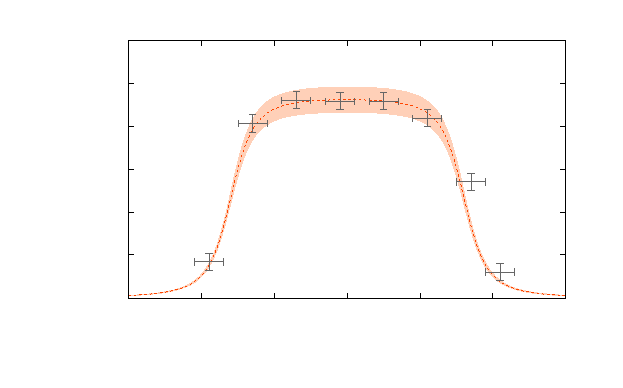
\includegraphics{camp-300-33}}%
    \gplfronttext
  \end{picture}%
\endgroup

	\caption{Camp magnètic al llarg de l'eix d'una bobina de 300 voltes, longitud \SI{16}{cm} i diàmetre \SI{3.3}{cm} per la que hi passa un corrent constant de \SI{1}{A}.}
	\label{fig:camp 300/33}
\end{figure}

\begin{figure}[tp]
	\sffamily \small
	\centering
	% GNUPLOT: LaTeX picture with Postscript
\begingroup
\sffamily \small
  \makeatletter
  \providecommand\color[2][]{%
    \GenericError{(gnuplot) \space\space\space\@spaces}{%
      Package color not loaded in conjunction with
      terminal option `colourtext'%
    }{See the gnuplot documentation for explanation.%
    }{Either use 'blacktext' in gnuplot or load the package
      color.sty in LaTeX.}%
    \renewcommand\color[2][]{}%
  }%
  \providecommand\includegraphics[2][]{%
    \GenericError{(gnuplot) \space\space\space\@spaces}{%
      Package graphicx or graphics not loaded%
    }{See the gnuplot documentation for explanation.%
    }{The gnuplot epslatex terminal needs graphicx.sty or graphics.sty.}%
    \renewcommand\includegraphics[2][]{}%
  }%
  \providecommand\rotatebox[2]{#2}%
  \@ifundefined{ifGPcolor}{%
    \newif\ifGPcolor
    \GPcolortrue
  }{}%
  \@ifundefined{ifGPblacktext}{%
    \newif\ifGPblacktext
    \GPblacktextfalse
  }{}%
  % define a \g@addto@macro without @ in the name:
  \let\gplgaddtomacro\g@addto@macro
  % define empty templates for all commands taking text:
  \gdef\gplbacktext{}%
  \gdef\gplfronttext{}%
  \makeatother
  \ifGPblacktext
    % no textcolor at all
    \def\colorrgb#1{}%
    \def\colorgray#1{}%
  \else
    % gray or color?
    \ifGPcolor
      \def\colorrgb#1{\color[rgb]{#1}}%
      \def\colorgray#1{\color[gray]{#1}}%
      \expandafter\def\csname LTw\endcsname{\color{white}}%
      \expandafter\def\csname LTb\endcsname{\color{black}}%
      \expandafter\def\csname LTa\endcsname{\color{black}}%
      \expandafter\def\csname LT0\endcsname{\color[rgb]{1,0,0}}%
      \expandafter\def\csname LT1\endcsname{\color[rgb]{0,1,0}}%
      \expandafter\def\csname LT2\endcsname{\color[rgb]{0,0,1}}%
      \expandafter\def\csname LT3\endcsname{\color[rgb]{1,0,1}}%
      \expandafter\def\csname LT4\endcsname{\color[rgb]{0,1,1}}%
      \expandafter\def\csname LT5\endcsname{\color[rgb]{1,1,0}}%
      \expandafter\def\csname LT6\endcsname{\color[rgb]{0,0,0}}%
      \expandafter\def\csname LT7\endcsname{\color[rgb]{1,0.3,0}}%
      \expandafter\def\csname LT8\endcsname{\color[rgb]{0.5,0.5,0.5}}%
    \else
      % gray
      \def\colorrgb#1{\color{black}}%
      \def\colorgray#1{\color[gray]{#1}}%
      \expandafter\def\csname LTw\endcsname{\color{white}}%
      \expandafter\def\csname LTb\endcsname{\color{black}}%
      \expandafter\def\csname LTa\endcsname{\color{black}}%
      \expandafter\def\csname LT0\endcsname{\color{black}}%
      \expandafter\def\csname LT1\endcsname{\color{black}}%
      \expandafter\def\csname LT2\endcsname{\color{black}}%
      \expandafter\def\csname LT3\endcsname{\color{black}}%
      \expandafter\def\csname LT4\endcsname{\color{black}}%
      \expandafter\def\csname LT5\endcsname{\color{black}}%
      \expandafter\def\csname LT6\endcsname{\color{black}}%
      \expandafter\def\csname LT7\endcsname{\color{black}}%
      \expandafter\def\csname LT8\endcsname{\color{black}}%
    \fi
  \fi
    \setlength{\unitlength}{0.0500bp}%
    \ifx\gptboxheight\undefined%
      \newlength{\gptboxheight}%
      \newlength{\gptboxwidth}%
      \newsavebox{\gptboxtext}%
    \fi%
    \setlength{\fboxrule}{0.5pt}%
    \setlength{\fboxsep}{1pt}%
\begin{picture}(5668.00,3400.00)%
    \gplgaddtomacro\gplbacktext{%
      \csname LTb\endcsname%%
      \put(946,704){\makebox(0,0)[r]{\strut{}\num{0}}}%
      \put(946,1199){\makebox(0,0)[r]{\strut{}\num{0.2}}}%
      \put(946,1694){\makebox(0,0)[r]{\strut{}\num{0.4}}}%
      \put(946,2189){\makebox(0,0)[r]{\strut{}\num{0.6}}}%
      \put(946,2684){\makebox(0,0)[r]{\strut{}\num{0.8}}}%
      \put(946,3179){\makebox(0,0)[r]{\strut{}\num{1}}}%
      \put(1078,484){\makebox(0,0){\strut{}\num{-15}}}%
      \put(1777,484){\makebox(0,0){\strut{}\num{-10}}}%
      \put(2476,484){\makebox(0,0){\strut{}\num{-5}}}%
      \put(3175,484){\makebox(0,0){\strut{}\num{0}}}%
      \put(3873,484){\makebox(0,0){\strut{}\num{5}}}%
      \put(4572,484){\makebox(0,0){\strut{}\num{10}}}%
      \put(5271,484){\makebox(0,0){\strut{}\num{15}}}%
    }%
    \gplgaddtomacro\gplfronttext{%
      \csname LTb\endcsname%%
      \put(198,1941){\rotatebox{-270}{\makebox(0,0){\strut{}$\mathsf{B \ (\si{mT})}$}}}%
      \put(3174,154){\makebox(0,0){\strut{}$\mathsf{z \ (\si{cm})}$}}%
    }%
    \gplbacktext
    \put(0,0){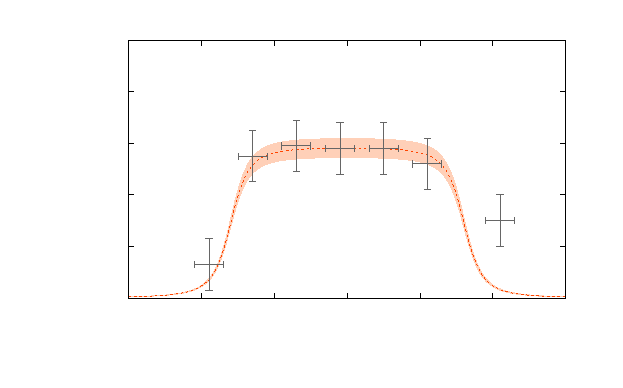
\includegraphics{camp-75-26}}%
    \gplfronttext
  \end{picture}%
\endgroup

	\caption{Camp magnètic al llarg de l'eix d'una bobina de 75 voltes, longitud \SI{16}{cm} i diàmetre \SI{2.6}{cm} per la que hi passa un corrent constant de \SI{1}{A}.}
	\label{fig:camp 75/26}
\end{figure}

\begin{figure}[tp]
	\sffamily \small
	\centering
	% GNUPLOT: LaTeX picture with Postscript
\begingroup
\sffamily \small
  \makeatletter
  \providecommand\color[2][]{%
    \GenericError{(gnuplot) \space\space\space\@spaces}{%
      Package color not loaded in conjunction with
      terminal option `colourtext'%
    }{See the gnuplot documentation for explanation.%
    }{Either use 'blacktext' in gnuplot or load the package
      color.sty in LaTeX.}%
    \renewcommand\color[2][]{}%
  }%
  \providecommand\includegraphics[2][]{%
    \GenericError{(gnuplot) \space\space\space\@spaces}{%
      Package graphicx or graphics not loaded%
    }{See the gnuplot documentation for explanation.%
    }{The gnuplot epslatex terminal needs graphicx.sty or graphics.sty.}%
    \renewcommand\includegraphics[2][]{}%
  }%
  \providecommand\rotatebox[2]{#2}%
  \@ifundefined{ifGPcolor}{%
    \newif\ifGPcolor
    \GPcolortrue
  }{}%
  \@ifundefined{ifGPblacktext}{%
    \newif\ifGPblacktext
    \GPblacktextfalse
  }{}%
  % define a \g@addto@macro without @ in the name:
  \let\gplgaddtomacro\g@addto@macro
  % define empty templates for all commands taking text:
  \gdef\gplbacktext{}%
  \gdef\gplfronttext{}%
  \makeatother
  \ifGPblacktext
    % no textcolor at all
    \def\colorrgb#1{}%
    \def\colorgray#1{}%
  \else
    % gray or color?
    \ifGPcolor
      \def\colorrgb#1{\color[rgb]{#1}}%
      \def\colorgray#1{\color[gray]{#1}}%
      \expandafter\def\csname LTw\endcsname{\color{white}}%
      \expandafter\def\csname LTb\endcsname{\color{black}}%
      \expandafter\def\csname LTa\endcsname{\color{black}}%
      \expandafter\def\csname LT0\endcsname{\color[rgb]{1,0,0}}%
      \expandafter\def\csname LT1\endcsname{\color[rgb]{0,1,0}}%
      \expandafter\def\csname LT2\endcsname{\color[rgb]{0,0,1}}%
      \expandafter\def\csname LT3\endcsname{\color[rgb]{1,0,1}}%
      \expandafter\def\csname LT4\endcsname{\color[rgb]{0,1,1}}%
      \expandafter\def\csname LT5\endcsname{\color[rgb]{1,1,0}}%
      \expandafter\def\csname LT6\endcsname{\color[rgb]{0,0,0}}%
      \expandafter\def\csname LT7\endcsname{\color[rgb]{1,0.3,0}}%
      \expandafter\def\csname LT8\endcsname{\color[rgb]{0.5,0.5,0.5}}%
    \else
      % gray
      \def\colorrgb#1{\color{black}}%
      \def\colorgray#1{\color[gray]{#1}}%
      \expandafter\def\csname LTw\endcsname{\color{white}}%
      \expandafter\def\csname LTb\endcsname{\color{black}}%
      \expandafter\def\csname LTa\endcsname{\color{black}}%
      \expandafter\def\csname LT0\endcsname{\color{black}}%
      \expandafter\def\csname LT1\endcsname{\color{black}}%
      \expandafter\def\csname LT2\endcsname{\color{black}}%
      \expandafter\def\csname LT3\endcsname{\color{black}}%
      \expandafter\def\csname LT4\endcsname{\color{black}}%
      \expandafter\def\csname LT5\endcsname{\color{black}}%
      \expandafter\def\csname LT6\endcsname{\color{black}}%
      \expandafter\def\csname LT7\endcsname{\color{black}}%
      \expandafter\def\csname LT8\endcsname{\color{black}}%
    \fi
  \fi
    \setlength{\unitlength}{0.0500bp}%
    \ifx\gptboxheight\undefined%
      \newlength{\gptboxheight}%
      \newlength{\gptboxwidth}%
      \newsavebox{\gptboxtext}%
    \fi%
    \setlength{\fboxrule}{0.5pt}%
    \setlength{\fboxsep}{1pt}%
\begin{picture}(5668.00,3400.00)%
    \gplgaddtomacro\gplbacktext{%
      \csname LTb\endcsname%%
      \put(946,704){\makebox(0,0)[r]{\strut{}\num{0}}}%
      \put(946,1323){\makebox(0,0)[r]{\strut{}\num{0.5}}}%
      \put(946,1942){\makebox(0,0)[r]{\strut{}\num{1}}}%
      \put(946,2560){\makebox(0,0)[r]{\strut{}\num{1.5}}}%
      \put(946,3179){\makebox(0,0)[r]{\strut{}\num{2}}}%
      \put(1078,484){\makebox(0,0){\strut{}\num{-15}}}%
      \put(1777,484){\makebox(0,0){\strut{}\num{-10}}}%
      \put(2476,484){\makebox(0,0){\strut{}\num{-5}}}%
      \put(3175,484){\makebox(0,0){\strut{}\num{0}}}%
      \put(3873,484){\makebox(0,0){\strut{}\num{5}}}%
      \put(4572,484){\makebox(0,0){\strut{}\num{10}}}%
      \put(5271,484){\makebox(0,0){\strut{}\num{15}}}%
    }%
    \gplgaddtomacro\gplfronttext{%
      \csname LTb\endcsname%%
      \put(198,1941){\rotatebox{-270}{\makebox(0,0){\strut{}$\mathsf{B \ (\si{mT})}$}}}%
      \put(3174,154){\makebox(0,0){\strut{}$\mathsf{z \ (\si{cm})}$}}%
    }%
    \gplbacktext
    \put(0,0){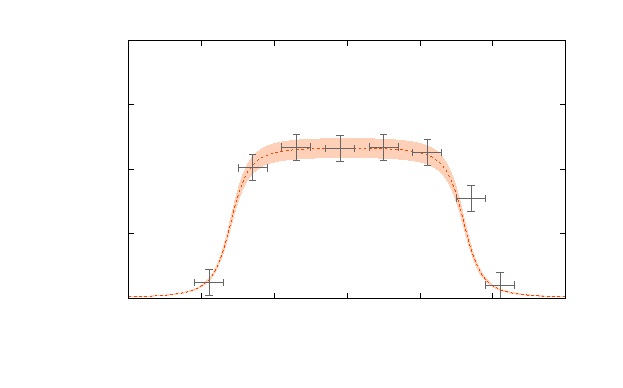
\includegraphics{camp-150-26}}%
    \gplfronttext
  \end{picture}%
\endgroup

	\caption{Camp magnètic al llarg de l'eix d'una bobina de 150 voltes, longitud \SI{16}{cm} i diàmetre \SI{2.6}{cm} per la que hi passa un corrent constant de \SI{1}{A}.}
	\label{fig:camp 150/26}
\end{figure}

\begin{figure}[tp]
	\sffamily \small
	\centering
	% GNUPLOT: LaTeX picture with Postscript
\begingroup
\sffamily \small
  \makeatletter
  \providecommand\color[2][]{%
    \GenericError{(gnuplot) \space\space\space\@spaces}{%
      Package color not loaded in conjunction with
      terminal option `colourtext'%
    }{See the gnuplot documentation for explanation.%
    }{Either use 'blacktext' in gnuplot or load the package
      color.sty in LaTeX.}%
    \renewcommand\color[2][]{}%
  }%
  \providecommand\includegraphics[2][]{%
    \GenericError{(gnuplot) \space\space\space\@spaces}{%
      Package graphicx or graphics not loaded%
    }{See the gnuplot documentation for explanation.%
    }{The gnuplot epslatex terminal needs graphicx.sty or graphics.sty.}%
    \renewcommand\includegraphics[2][]{}%
  }%
  \providecommand\rotatebox[2]{#2}%
  \@ifundefined{ifGPcolor}{%
    \newif\ifGPcolor
    \GPcolortrue
  }{}%
  \@ifundefined{ifGPblacktext}{%
    \newif\ifGPblacktext
    \GPblacktextfalse
  }{}%
  % define a \g@addto@macro without @ in the name:
  \let\gplgaddtomacro\g@addto@macro
  % define empty templates for all commands taking text:
  \gdef\gplbacktext{}%
  \gdef\gplfronttext{}%
  \makeatother
  \ifGPblacktext
    % no textcolor at all
    \def\colorrgb#1{}%
    \def\colorgray#1{}%
  \else
    % gray or color?
    \ifGPcolor
      \def\colorrgb#1{\color[rgb]{#1}}%
      \def\colorgray#1{\color[gray]{#1}}%
      \expandafter\def\csname LTw\endcsname{\color{white}}%
      \expandafter\def\csname LTb\endcsname{\color{black}}%
      \expandafter\def\csname LTa\endcsname{\color{black}}%
      \expandafter\def\csname LT0\endcsname{\color[rgb]{1,0,0}}%
      \expandafter\def\csname LT1\endcsname{\color[rgb]{0,1,0}}%
      \expandafter\def\csname LT2\endcsname{\color[rgb]{0,0,1}}%
      \expandafter\def\csname LT3\endcsname{\color[rgb]{1,0,1}}%
      \expandafter\def\csname LT4\endcsname{\color[rgb]{0,1,1}}%
      \expandafter\def\csname LT5\endcsname{\color[rgb]{1,1,0}}%
      \expandafter\def\csname LT6\endcsname{\color[rgb]{0,0,0}}%
      \expandafter\def\csname LT7\endcsname{\color[rgb]{1,0.3,0}}%
      \expandafter\def\csname LT8\endcsname{\color[rgb]{0.5,0.5,0.5}}%
    \else
      % gray
      \def\colorrgb#1{\color{black}}%
      \def\colorgray#1{\color[gray]{#1}}%
      \expandafter\def\csname LTw\endcsname{\color{white}}%
      \expandafter\def\csname LTb\endcsname{\color{black}}%
      \expandafter\def\csname LTa\endcsname{\color{black}}%
      \expandafter\def\csname LT0\endcsname{\color{black}}%
      \expandafter\def\csname LT1\endcsname{\color{black}}%
      \expandafter\def\csname LT2\endcsname{\color{black}}%
      \expandafter\def\csname LT3\endcsname{\color{black}}%
      \expandafter\def\csname LT4\endcsname{\color{black}}%
      \expandafter\def\csname LT5\endcsname{\color{black}}%
      \expandafter\def\csname LT6\endcsname{\color{black}}%
      \expandafter\def\csname LT7\endcsname{\color{black}}%
      \expandafter\def\csname LT8\endcsname{\color{black}}%
    \fi
  \fi
    \setlength{\unitlength}{0.0500bp}%
    \ifx\gptboxheight\undefined%
      \newlength{\gptboxheight}%
      \newlength{\gptboxwidth}%
      \newsavebox{\gptboxtext}%
    \fi%
    \setlength{\fboxrule}{0.5pt}%
    \setlength{\fboxsep}{1pt}%
\begin{picture}(5668.00,3400.00)%
    \gplgaddtomacro\gplbacktext{%
      \csname LTb\endcsname%%
      \put(946,704){\makebox(0,0)[r]{\strut{}\num{0}}}%
      \put(946,1013){\makebox(0,0)[r]{\strut{}\num{0.5}}}%
      \put(946,1323){\makebox(0,0)[r]{\strut{}\num{1}}}%
      \put(946,1632){\makebox(0,0)[r]{\strut{}\num{1.5}}}%
      \put(946,1942){\makebox(0,0)[r]{\strut{}\num{2}}}%
      \put(946,2251){\makebox(0,0)[r]{\strut{}\num{2.5}}}%
      \put(946,2560){\makebox(0,0)[r]{\strut{}\num{3}}}%
      \put(946,2870){\makebox(0,0)[r]{\strut{}\num{3.5}}}%
      \put(946,3179){\makebox(0,0)[r]{\strut{}\num{4}}}%
      \put(1078,484){\makebox(0,0){\strut{}\num{-15}}}%
      \put(1777,484){\makebox(0,0){\strut{}\num{-10}}}%
      \put(2476,484){\makebox(0,0){\strut{}\num{-5}}}%
      \put(3175,484){\makebox(0,0){\strut{}\num{0}}}%
      \put(3873,484){\makebox(0,0){\strut{}\num{5}}}%
      \put(4572,484){\makebox(0,0){\strut{}\num{10}}}%
      \put(5271,484){\makebox(0,0){\strut{}\num{15}}}%
    }%
    \gplgaddtomacro\gplfronttext{%
      \csname LTb\endcsname%%
      \put(198,1941){\rotatebox{-270}{\makebox(0,0){\strut{}$\mathsf{B \ (\si{mT})}$}}}%
      \put(3174,154){\makebox(0,0){\strut{}$\mathsf{z \ (\si{cm})}$}}%
    }%
    \gplbacktext
    \put(0,0){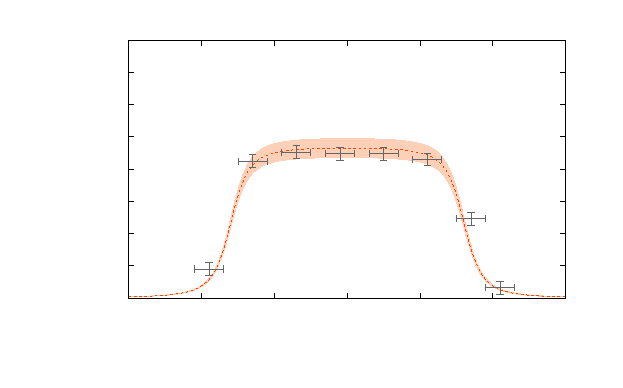
\includegraphics{camp-300-26}}%
    \gplfronttext
  \end{picture}%
\endgroup

	\caption{Camp magnètic al llarg de l'eix d'una bobina de 300 voltes, longitud \SI{16}{cm} i diàmetre \SI{2.6}{cm} per la que hi passa un corrent constant de \SI{1}{A}.}
	\label{fig:camp 300/26}
\end{figure}

A les \cref{fig:camp 300/33,fig:camp 75/26,fig:camp 150/26,fig:camp 300/26} hi ha representat el mòdul del camp magnètic al llarg de l'eix de les bobines mesurades durant l'experiment---calculat a partir de l'\cref{eq:camp bobina} i amb el corresponent marge d'incertesa--- aixì com els punts corresponents a les mesures realitzades

Tal i com es pot apreciar, al llarg de l'eix les mesures obtingudes s'ajusten molt bé a la prediccío teòrica. Això és d'esperar ja que a l'interior d'una bobina el camp és pràcticament constant. Als extrems, però, les dades experimentals no s'hi ajusten tant. Una explicació és que en el nostre cas l'acabament real de les bobines era complicat de detectar. A més pel que fa als valors teòrics aquests disminueixen molt sobtadament a l'exterior de la bobina. Si es tenen en compte aquests dos factors és senzill comprendre les possibles discrepàncies als extrems de les bobines.

\section{Conclusions}
En general els resultats obtinguts han estat satisfactoris. S'ha observat empíricament al llarg de tota la pràctica els fets que s'havien demostrat de manera teòrica. El camp magnètic al centre d'una espira disminueix a mesura que augmenta el radi d'aquesta i ho fa com $\frac{1}{R}$ amb $R$ el radi de l'espira. S'ha comprovat també empíricament l'augment lineal del camp al centre d'un conjunt d'espires amb la quantitat d'espires. Aquest últim fet ha estat provat per conjunts de $1$, $2$ i $3$ espires. Les observacions han portat també a concloure que el camp magnètic al centre d'una bobina augmenta en apropar-se al centre i és màxim en aquest. El fet que el camp magnètic creat per una bobina on hi circula una certa intensitat augmenta amb el nombre de voltes, ha estat provat també de manera satisfactòria. Finalment s'ha calculat empíricament la permeabilitat magnètica $\mu_{0}$ i s'ha obtingut una bona aproximació d'aquesta.




